\section{The California Report Card}
\subsection{System Description}
The California Report Card (CRC) is a web application that allows participants to advise the state government on timely policy issues.
The CRC is divided into two phases: assessment and deliberation.
In the assessment phase, participants grade the state's policies on a scale from A+ to F on six issues with a slider.
Participants have the option to skip any issue.	
After a participant's first response, the median grade for all participants is revealed. 
The slider, is however, still active and participants have the option to change their grades.
This process is illustrated in Figure \ref{grading-1}.
In the deliberation phase, participants submit textual suggestions on future issues to include in the report card.
In this work, we focus on the assesment phase and defer an analysis of biases in the deliberation phase to future work.

\subsubsection{The Six Issues}
The six issues were:
\begin{itemize}
\item Implementation of the Affordable Care Act ("Obamacare")
\item Quality of K-12 public education
\item Affordability of state colleges and universities
\item Access to state services for undocumented immigrants
\item Laws and regulations regarding recreational marijuana
\item Marriage rights for same-sex partners
\end{itemize}
These issues were posed in a constant sequential order with the same input scale (A+ to F).
The issues were chosen to be timely and relevant to a majority of Californians.

\subsection{Dataset and Experimental Setup}
For each of the six issues, the report card collected around 1700 distinct inputs (both grades and skips). 
Grades were recorded every time the slider was released.
The slider for the grades was discretized into 13 parts (A+, A, A-,...).

For analysis, we mapped these 13 grades onto a scale from 0 to 1, with 1 being an A+ and 0 being an F.
For each participant $p_j$, we associate a 3-tuple of grades ($g_i[j]$, $m[j]$, $g_f[j]$) which reprsent the initial grade, median observed by the participant, and the final grade.
To control for random changes or artifacts of the input device (eg. the slider stops), we counted changes
that spanned a minimum time threshold of 3 seconds.
With this definition, between 10\% and 20\% of the final grades involved at least one grade change.
A detailed breakdown for each issue is illustrated in Figure \ref{grading-2}.

We further conducted a reference survey through Survey Monkey asking the same questions (including the option to skip) without the median grade feedback. 
The reference survey had a sample size of 611 participants.

\begin{figure}[h!]
  \centering
    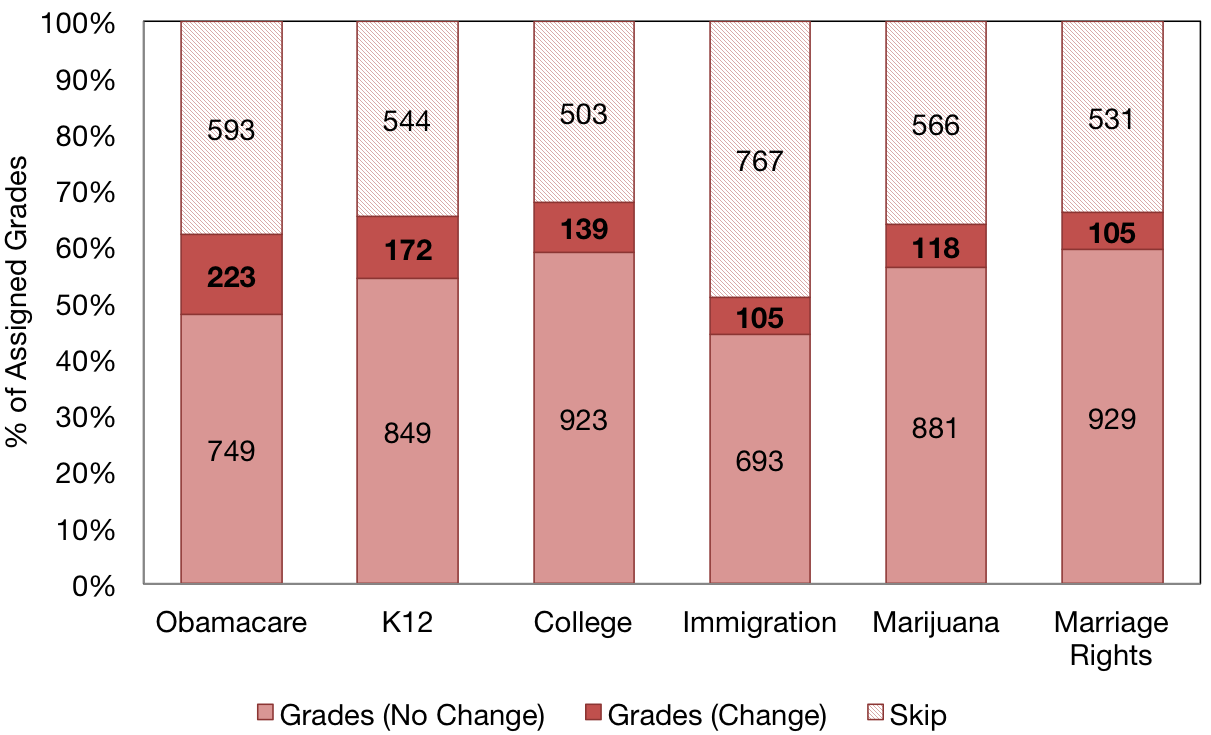
\includegraphics[width=\columnwidth]{../plots/grading-behavior-1.png}
      \caption{Breakdown of Activity in CRC Assesment.}
      \label{grading-2}
\end{figure}
